% Setup - do not change
\documentclass[11pt]{article}
\usepackage[top=0.9in, left=0.9in, bottom=0.9in, right=0.9in]{geometry} 
\usepackage{parskip}

\usepackage[english]{babel}
\usepackage[utf8]{inputenc}
\usepackage{amsmath,amsthm,amssymb,graphicx,pdfpages,lipsum,hyperref}
\usepackage[none]{hyphenat}
\usepackage{csquotes}
\usepackage{subfig}
\usepackage{hyperref}


\setlength\parindent{0pt}
%%%%%%%%%%%%%%%%%%%%%%%%%%%%%%%%%%%%%%%%%%%%%%%%%%%%%%%%%%%%%%%%%%%
% add other packages here if required

%% Bibliography are specified in this file. You can also choose inline bib style if you want to. But make sure your citation style is consistent (and proper)
% For more details on citation: https://library.unimelb.edu.au/recite
\usepackage[sorting = none]{biblatex}
\addbibresource{references.bib}

%%%%%%%%%%%%%%%%%%%%%%%%%%%%%%%%%%%%%%%%%%%%%%%%%%%%%%%%%%%%%%%%%%% the '%' symbol denotes comments

% Begin document creation
% DELETE THE \lipsum PLACEHOLDERS WHEN YOU BEGIN
\title{\textbf{Tipping prediction for Yellow Taxis in New York in relation to New York Knicks playing }}
\author{
Dustin Edgar Tano \\
Student ID: 1188678 \\
%% Replace the link with your github repo
% 1. Remember to escape underscore (\_) in the link.
% 2. Remember to include the commit you want to submit in the link
\href{https://github.com/MAST30034-Applied-Data-Science/mast30034-project-1-dustintano10.git}{Github repo with commit}
}

\begin{document}
\maketitle

\section{Introduction}
% Link to a 30 min tutorial if you require revision: https://www.overleaf.com/learn/latex/Learn_LaTeX_in_30_minutes

The New York Knicks are the most valuable team in the NBA with a value of 5.8 billion dollars \cite{2021-22mostvaluedteam}. Being the most valuable team comes with popularity as they are the 2nd most popular sports team behind the New York Yankees based on facebook followers \cite{2020mostpopularNYteams}. This report should be viewed in the perspective of a yellow taxi driver with the objective of predicting the amount of tips while the New York Knicks are playing.

Through various preprocessing, outlier analysis and plots, a linear regression model which got its features selected through LASSO and a Ridge regression model were decided for predictions. Through these methods it was found that non of the features from the external dataset had any relevance in predicting tip amount showing that the Knicks do not have any influence in tipping. 

This report assumes that the effects of the Knicks games and it's results has influence throughout the whole day, not only after the Knicks games are finished. Friday is also assumed to be a weekday not a weekend as some may interpret this differently.   

% You can have \section{}, \subsection{}, and \subsubsection{}
\section{Data-Processing}

\subsection{Data-set}
The report primarily uses data published by the NYC \& Taxi limousine company \cite{taxidataset}. This data set records statistics from both taxis and for hire vehicles in an hourly basis per day for every year. Yellow taxi was chosen since it has a clear feature for tips unlike the for-hire vehicles while green taxis are not considered since it does not cover the whole of New York. The size of the yellow taxi data set before preprocessing is 55,274,200 records. The NYC \& Taxi limousine company also provides files describing shapes of each location within New York. The purpose of these particular files are for the geospatial visualisations. 

Other than the Yellow Taxi data set, an NBA attendance data set for the season of 2018-19 \cite{nbaAttendancedataset} is used since the research relates to the New York Knicks playing. The data set is retrieved from basketball-reference which is a website that stores statistics related to anything basketball. The data set has a size of 1278 records. From this data set the features Start (ET) and Attendance would be used in the model for tip prediction. Further engineered features from this data set will also contribute to the model. 

\subsection{Range Selection}
The range of time chosen is from October 2018 to April 2019. This coincides with the time frame of a single full NBA season not counting the playoffs. Playoffs are not counted since in this particular season the Knicks did not make the playoffs. Also the 2018-19 NBA season was the last NBA season before the COVID-19 pandemic ravaged the world and the NBA has only recently started accepting full attendance to their stadiums. 

\subsection{Cleaning}
This section outlines the methods used to remove outliers, keep features consistent with the data dictionary and filtering out features that were not relevant for analysis

\subsubsection{Yellow Taxi}
Yellow Taxi underwent these steps for cleaning:
\begin{itemize}
    \item{Filter out Vendor ID which is not 1 or 0, filtered passenger count where it is greater than 0 }
    \item{Filtered payment type where it is 1, tips are only counted for those paying with credit card}
    \item{Filtered rate codes where it is 0 or 1, other rate codes makes small amount of data set}
    \item{Filtered trips where it starts in the month of October}
    \item{Filtered trips distance where it is greater than 0, filtered the pickup and drop off locations to be within the range of 1-263}
    \item{Filtered fare amount to start at \$ 2.50, this follows the initial charge stated in the NYC Taxi \& Limousine website\cite{initialFareAmount} }
    \item{Filtered trip time where it is more than 2 minutes, trips less than 2 minutes not reasonable}
    \item{Removed extra, mta tax, congestion surcharge, airport fee, improvement surcharge, passenger count and store and fwd flag columns as they are not relevant for analysis}
    \item{Removed outliers for fare amount. Outliers determined by finding the 1st and 3rd quantiles, getting the IQR and finally filtering anything greater or less than 1.5*IQR }
    \item{Filtered instances where the pickup and dropoff dates are different, research is only focused on days Knicks are playing and there are no games where the Knicks play back to back at home}

\end{itemize}
\subsubsection{NBA Attendance}
The NBA Attendance dataset is a small one thus only a handfull of steps were done for cleaning. Remove the unnamed columns and notes, renamed the Attend. column to Attendance. Filtered Home to New York Knicks only since research revolves around the Knicks playing at Home. Removed the Home, Away, PTS, PTS.1 and Arena columns, considered irrelevant. Converted the Date column to have same format to date in taxi data set.

\subsection{Feature engineering, data size and sampling}
This section outlines the formation of new features, the data size after pre-processing and the way data is aggregated and sampled.

\subsubsection{Feature engineering Yellow Taxi}
Features created from Yellow Taxi:
\begin{itemize}
    \item{Created a column called is weekend to see if the date is a weekend or not}
    \item{Created a column called trip length which records time taken for a trip in minutes}
    \item{Created a column called is weekend binary, which converts true and false into 1 and 0}
    \item{Created columns pickup hour and dropoff hour which records pickups and dropoffs in an hourly basis}
\end{itemize}

\subsubsection{Feature engineering NBA Attendance}
Features created from NBA Attendance:
\begin{itemize}
    \item{Created a Win column which indicates if the Knicks won or lost the game}
    \item{Created a day,month and year columns which are then combined to produce a new version of the date column which is then converted to have the same format with the yellow taxi}
    \item{Created a margin victory/loss column which shows how big the score margin is. If it's negative it indicates the amount of points needed for the Knicks to tie the game}
    \item{Converted the Start(ET) column into categorical numbers (ex: 1, 2, 3). This would be used for modelling}

\end{itemize}

\subsubsection{Data Size}
After cleaning the respective data sets we get 32,399,765 instances for the taxi data set and only a mere 41 instances for the NBA Attendance data set. This is not a surprise for the NBA Attendance data set since the New York Knicks only played 41 games at home in an 82 game season. 

The 2 data sets are then joined on the pickup date of the Yellow Taxi with the Date of the NBA Attendance. After the join the combined data set has a size of 6,165,834 instances. These are instances of taxi data that exists in the days the Knicks play after undergoing pre-processing.

\subsubsection{Sampling}
Due to limitations in computer specifications a full distribution of the data set could not be used for analysis. Thus 10\% of the full data set is taken and used for some aspects of analysis. Other aggregations are used for analysis such as hourly aggregations, Start time aggregation and Location aggregations for both pick ups and drop offs.

\section{Analysis}
In order to predict tip amount, relationships between our variables and tip amount are investigated. This is done through visualisation of the data that has been aggregated and data which have been sampled. The following subsections describes the processes. 

\subsection{Continuous variable analysis}
Starting of, the continuous variables of our combined data set are studied. These being fare amount, total amount, tolls amount, trip distance, trip length, Attendance and margin victory\\loss. Their correlations are calculated then presented as a correlation matrix.
\begin{figure}[h]
    % change the scale multiplier to make the figures smaller or larger
    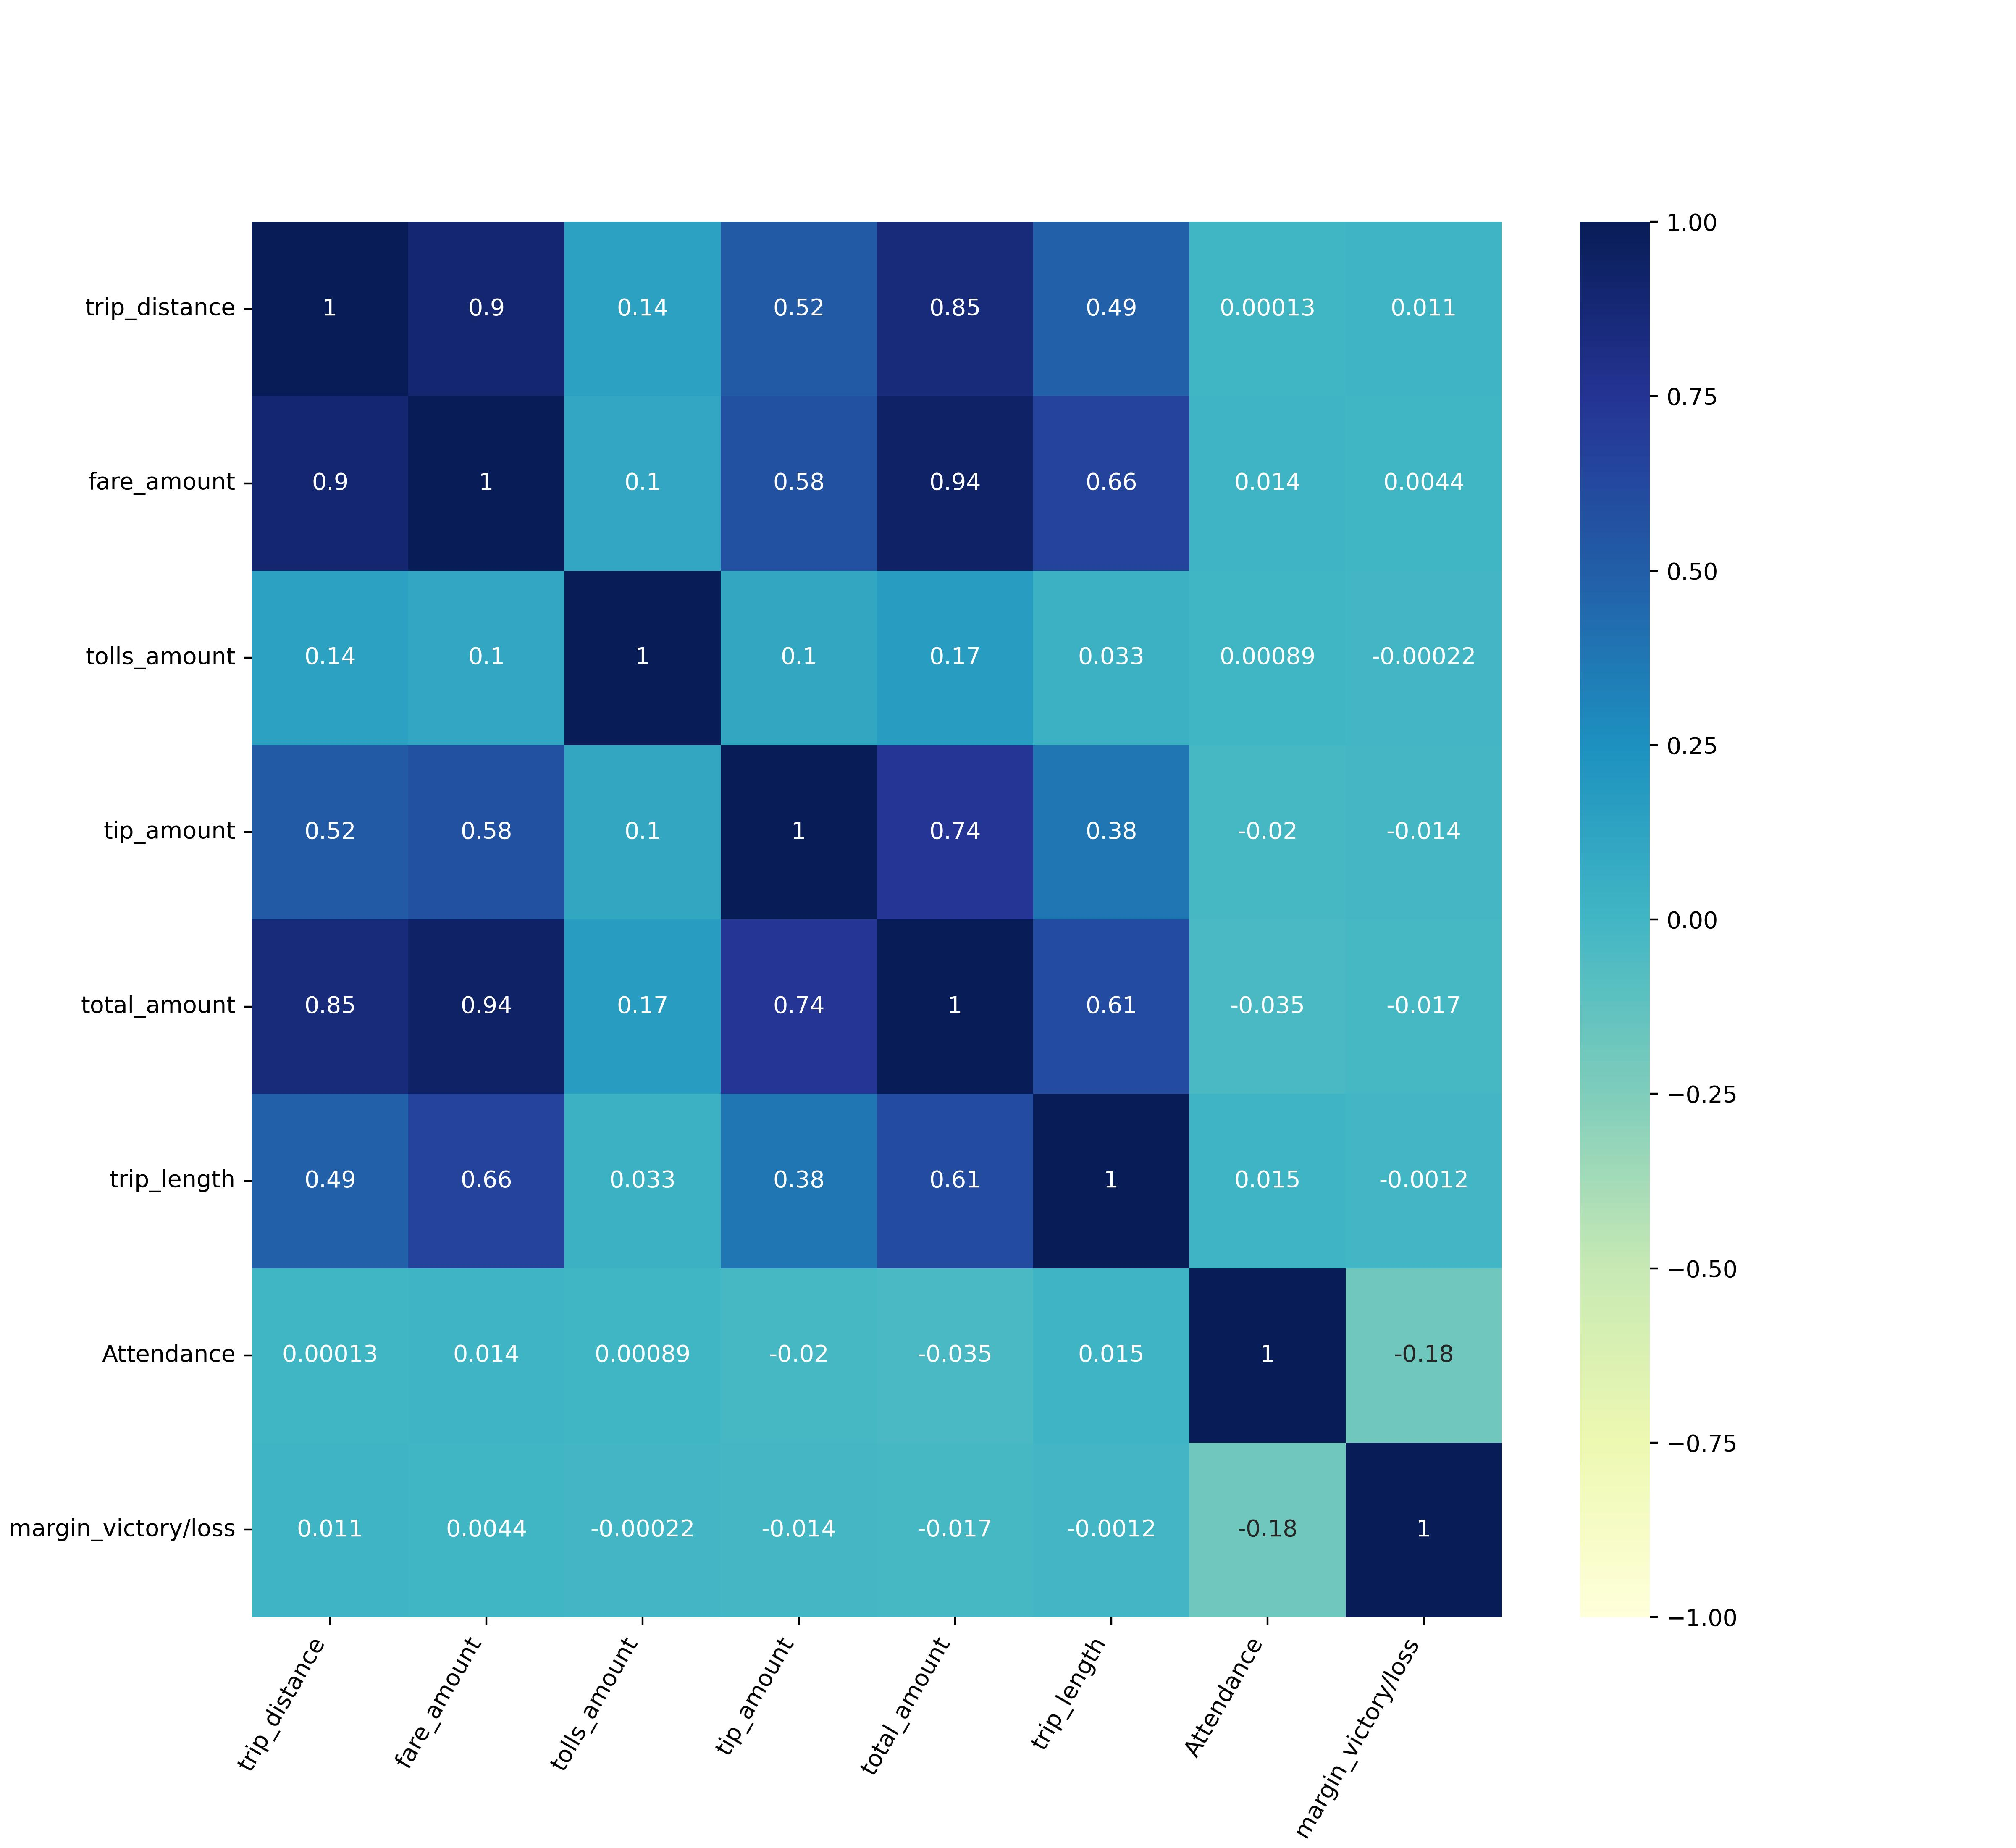
\includegraphics[height = 13 cm, width = 18 cm]{plots/correlation_matrix.jpeg}
    % this ensures your figures are centered where possible
    \centering
    \caption{Correlation matrix of continuous variables} % refer to this image as (Figure 1)
\end{figure}

Based on the correlation matrix, tip amount has strong correlations with total amount, fare amount and trip distance. Tolls amount and trip length surprisingly have weak correlations with tip amount. The idea of a longer trip meaning a higher tip thus is debunked from the matrix. Continuous variables from our NBA attendance data set apparently have very weak or even no correlation to our tip amount these being attendance and margin victory/loss. This is unsurprising considering that there really is no logical reasoning for the score margin to affect tip behaviour. Same as attendance, this specific variable instead could maybe be related to the trip demand.

\begin{figure}[h]
    \centering
    \begin{minipage}[b]{0.45\textwidth}
        \centering
        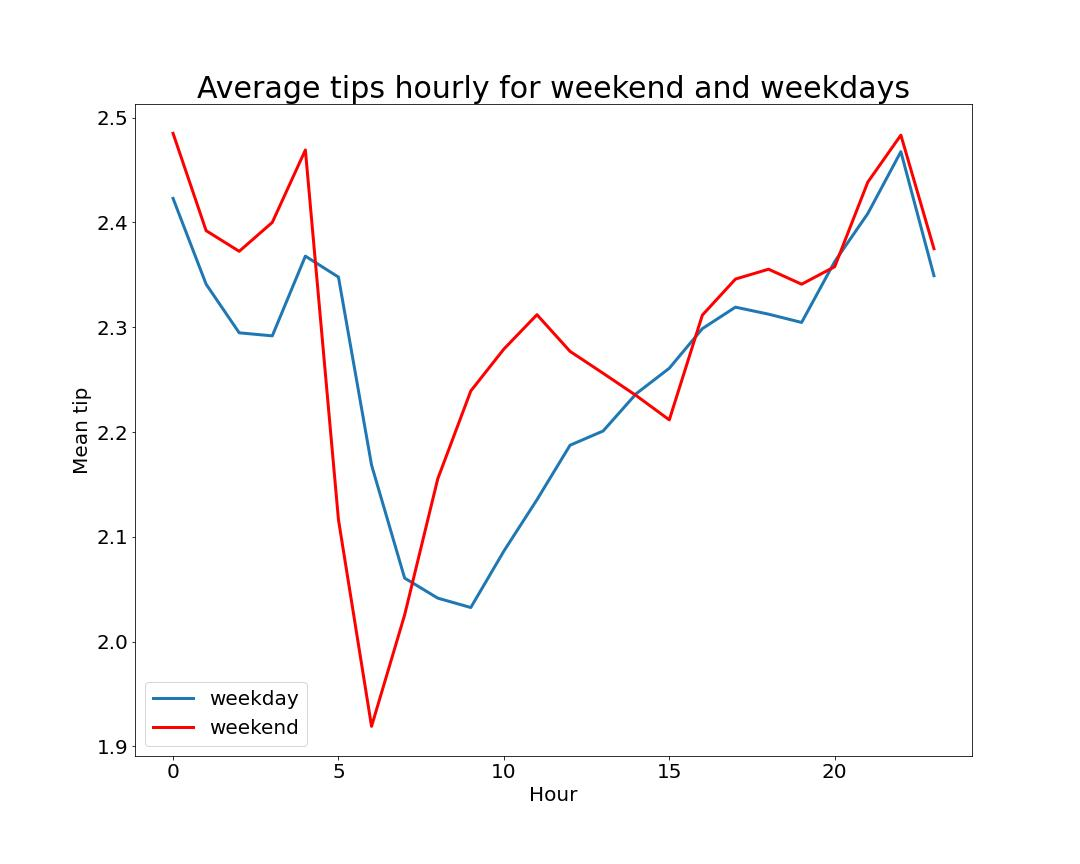
\includegraphics[width=\textwidth]{plots/time_series_plot_weekday_weekend.jpeg}
        \subfloat{(a) Weekend vs Weekday}
    \end{minipage}
    \hfill
    \begin{minipage}[b]{0.45\textwidth}
        \centering
        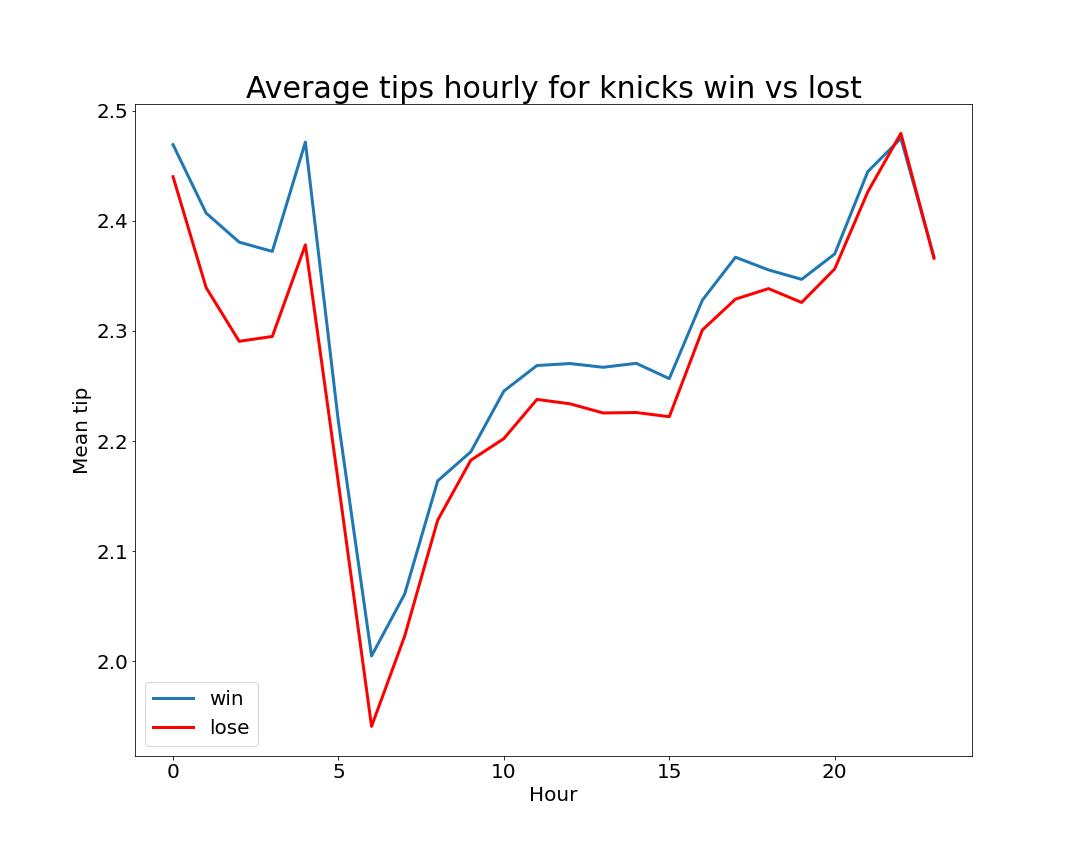
\includegraphics[width=\textwidth]{plots/time_series_plot_win_lost.jpeg}
        \subfloat{(b) Win vs Lost}
    \end{minipage}
    \hfill
    \caption{Time series plots for respective discrete variables}
\end{figure}

\subsection{Categorical attributes}
For the is weekend and wins features since they are discrete, including them in the correlation matrix won't work. Thus for the is weekend and wins features, time series plots were created while for the Start(ET) feature a bar plot was created. Since New York could be seen as a bustling city, time is assumed to have an effect on how passengers tip in terms of amount. 

From figure 2.a we could see that the tips for weekends are higher then weekends for most of the day. This is not surprising since people tend to go out more in the weekends and spend more. An interesting trend seen from this time series plot is that in hours from around 5-7 AM the tip amount for weekends plummets compared to weekdays showing that people don't generally go out in these early times when there is no work.

For figure 2.b, the trend is not as clear. It may look like the Knicks winning means a higher average tip hourly but the difference is very slight. There are certain hours of 
the day where it is clear like from 10-15.

\begin{figure}[h]
    % change the scale multiplier to make the figures smaller or larger
    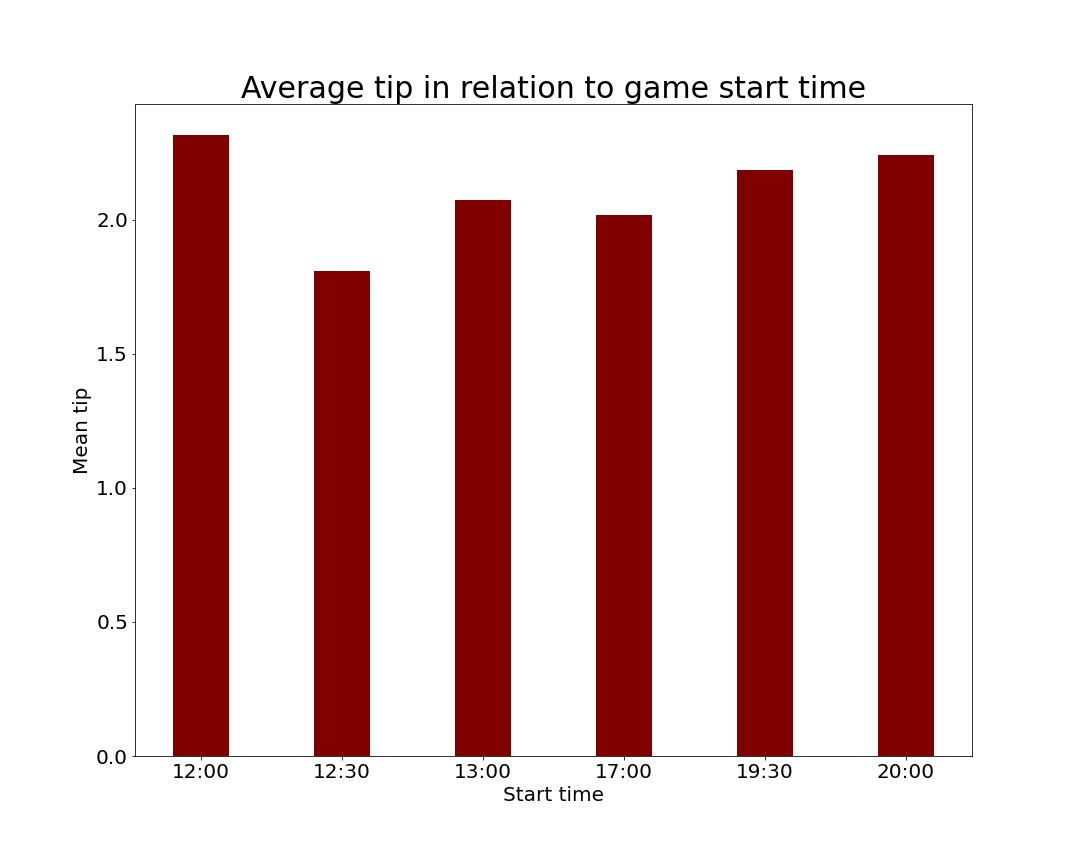
\includegraphics[height = 8 cm , width = 13 cm]{plots/bar_plot_gamestart.jpeg}
    % this ensures your figures are centered where possible
    \centering
    \caption{Bar plot on mean tip in relation to game start time} % refer to this image as (Figure 1)
\end{figure}
Figure 3 shows that the game start time does not have any correlation for tip amount. This can be seen from its trends where the only clear trend is that when the game starts at 12:30 the mean tip amount is at its lowest


\subsection{Geospatial Analysis}
This section describes and shows the mean tip amount per area of New York through the visualisation of heatmaps in the map of New York. 

\begin{figure}[t]
    \centering
    \begin{minipage}[t]{0.45\textwidth}
        \centering
        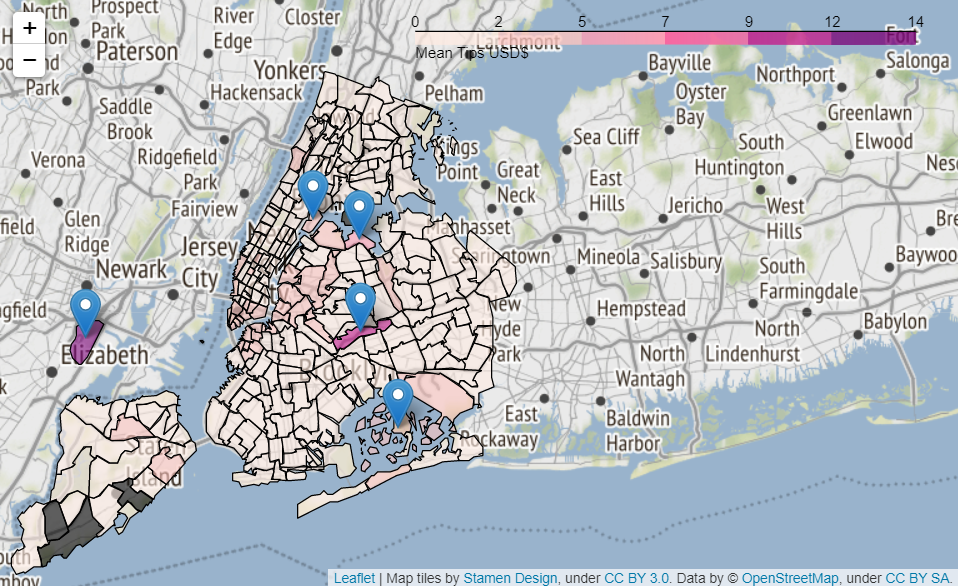
\includegraphics[height = 8 cm, width = 9 cm]{plots/Geoplot_PU_tip.png}
        \subfloat{(a) Mean tips for Pick up location}
    \end{minipage}
    \hfill
    \begin{minipage}[t]{0.45\textwidth}
        \centering
        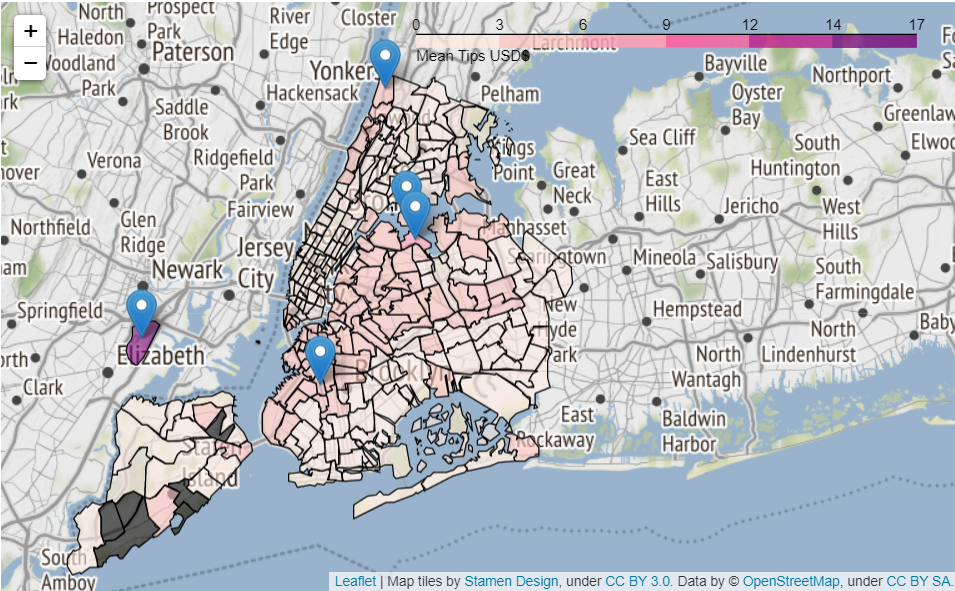
\includegraphics[height = 8 cm, width = 9 cm]{plots/Geoplot_DO_tip.png}
        \subfloat{(b) Mean tips for drop off location}
    \end{minipage}
    \hfill
    \caption{Geospatial plots for both Pick up and Drop off locations}
\end{figure}

From the geo-spatial plots we see that some areas have a very high tip average for both the pickup and drop off locations. The markers shown are the top 5 areas which has the highest average tip in New York.

\begin{table}[h!]
\centering
\begin{tabular}{||c c||} 
 \hline
 Pickup location & Mean tip  \\ [0.5ex] 
 \hline\hline
 Newark Airport & 14.230 \\ 
 \hline
 Forest Park/Highland Park & 10.666 \\
 \hline
 LaGuardia Airport & 5.376\\
 \hline
 Jamaica Bay & 4.373\\
 \hline
 Randalls Island & 3.958\\ [0.5 ex] 
 \hline
\end{tabular}
\caption{Top 5 locations in terms of mean tip for Pick up location}
\end{table}

\begin{table}[h!]
\centering
\begin{tabular}{||c c||} 
 \hline
 Drop off location & Mean tip  \\ [0.5ex] 
 \hline\hline
 Newark Airport & 17.285 \\ 
 \hline
 Laguardia Airport & 6.098 \\
 \hline
 Rikers Island & 4.660\\
 \hline
 Riverdale/North Riverdale/Fieldston & 4.567\\
 \hline
 Windsor Terrace & 4.507\\ [0.5 ex] 
 \hline
\end{tabular}
\caption{Top 5 locations in terms of mean tip for Drop Off location}
\end{table}

From these 2 tables we can see that Newark Airport is the top location in terms of tip amount. The spread for pickup location is way more spreadout as the top 2 locations have values that are so far apart from the rest. While for the drop off locations, the spread is more reasonable as from number 2 below the values are not far apart. It could be assumed that the top 2 areas in the pickup location are outliers while the number 1 earning location for the Drop off location is an outlier.

\section{Modelling}
For modelling since the goal is to predict the continuous variable tip amount, A linear regression model is chosen for this. Another model being used is the Ridge regression model and the LASSO model which would be used for feature selection in the linear regression model. All these models are adapted from the tutorial notebook given\cite{modelreference}

\subsection{Linear regression}
Linear regression is a statistical model which describes the dependent variable y with one or more independent variables x. This is generally used for prediction of a variable from another variable.This is chosen since it is a model which is easy to implement, quick to train and it works well with continuous variables. The equation it follows is: 
\begin{equation}
Y_i = \beta_0 + \beta_1 X_i
\end{equation}
The \begin{math} Y_i \end{math} variable represents the dependent variable the \begin{math} \beta_0 \end{math} variable represents the constant, the \begin{math} \beta_1 \end{math} variable represents the coefficient and the \begin{math} X_i \end{math} variable represents the independent variable.

\subsection{LASSO regression}
The LASSO regression follows the formula 
\begin{equation}
\label{eq:LASSO OLS}
\hat\beta^* = \text{argmin}_{\beta \in \mathcal{B}}(Y-X\beta)^T(Y-X\beta) + \lambda|\beta|_1
\end{equation}
It uses the L1 regularization term which means that it adds a penalty equal to the absolute value of the magnitude coefficient. Larger penalties means values closer to 0 thus could be used for feature selection in the Linear model. Sparse models are able to be created from this.

\subsection{Ridge regression}
The Ridge regression follows the formula
\begin{equation}
\label{eq:Ridge}
\hat\beta^* = \text{argmin}_{\beta \in \mathcal{B}}(Y-X\beta)^T(Y-X\beta) + \frac{1}{2}\lambda|\beta|_2^2
\end{equation}
Instead of using the L1 regularization term, it uses the L2 regularization term. This term adds a penalty equal to the square of the magnitude of coefficients. This results in all the other coefficients to be shrunk by the same factor. Unlike the LASSO regression sparse models are not achievable.

\subsection{Prediction}
\begin{table}[h]
\centering
\begin{tabular}{||c c c c ||} 
 \hline
 Type & RMSE & MAE & MSE  \\ [0.5ex] 
 \hline\hline
 Train & 0.3344 & 0.2704 & 0.1118 \\ 
 \hline
 Test & 0.3544 &  0.2909 & 0.1256 \\
 \hline
\end{tabular}
\caption{Evaluation metrics for Linear regression model}
\end{table}

\begin{table}[h]
\centering
\begin{tabular}{||c c c c ||} 
 \hline
 Type & RMSE & MAE & MSE  \\ [0.5ex] 
 \hline\hline
 Train & 0.9097 & 0.4600 & 0.8275 \\ 
 \hline
 Test &  0.9479 &  0.4223 & 0.8986 \\
 \hline
\end{tabular}
\caption{Evaluation metrics for Ridge regression model}
\end{table}
Before fitting the model, the data set is split into a train and test set. Since the goal is prediction the first game in 2019 is chosen as the test set while all game days in 2018 are chosen as the training set. Then through ridge regression of the full model we select the features. The features removed are Attendance, Win, margin victory/loss,trip length, PU and DOLocationID and finally Start(ET). The fact that all variables from the external data set are removed is not a surprise considering there was no real correlation from the prior analysis. The surprising removal is trip length.

After feature selection we fit the reduced model into the linear regression and also fit the full model into the ridge regression. Evaluation metrics were then formed for the train and test per respective model.

\subsection{Discussion}
Table's 3 and 4 are Evaluation summaries for the linear and ridge regression models respectively. The metrics chosen are Root mean square error (RMSE), Mean absolute error (MAE) and Mean square error (MSE). The MSE is the average of the squared difference between the predicted and actual value. The RMSE is the square root of the mean of the square of all the errors, this is a good accuracy indicator for error forecasting. The MAE is the average difference between target value and value predicted. 

Overall it can be seen that the Linear model performs better than the Ridge regression model. This could be seen from the lower RMSE,MAE and MSE values when compared. This is not surprising considering the ridge regression model shrinks its coefficient making it perform worst. However these very low values show strong signs in the possibilities of the data being over fitted on the reduced Linear regression model so even though it performs substantially better than Ridge the reduced Linear regression model may not be the best performing model. 

\section{Recommendations}
Through the analysis and modelling that has been undertook, it could be said that New York Knicks games have no influence in tip amounts. It is seen through the plots created that there are no correlations or significant trends supporting the influences of the Knicks. It is not surprising considering the research uses the assumption that the influences were to happen throughout the day when in reality it won't. It is more realistic to see the influences of the Knicks in taxi demand rather than tips. Since in the end the tips are mostly just influenced by the features from the taxi dataset alone. 

Instead of the assumption of the influences happening the whole day it is recommended to just study the influences after the game ends which would be usually 2 hours after the start time. Possibly the correlations and trends may appear more. Also it is recommended that more measures are taken in outlier removal. As seen in the geo-spatial analysis the high mean tips for certain areas could be because of the short amount of trips taken to and from that area. The area locations should also be one hot encoded instead of acting as a continous variable, more information could be obtained from that. The outliers might be one the driving force on why the linear regression model is overfitted.



\clearpage

% BEGIN REFERENCES SECTION
\printbibliography

\end{document}